\chapter{Desenvolvimento}
No sentido de melhorar a inserção do projeto Pensando o Direito e correlatos, 
abaixo estão descritas algumas iniciativas que visam uma maior integração em
termos de processos de comunicação e outras que podem ajudar a embasar futuros
estudos e iniciativas.

\section{Redes Sociais privadas}
De acordo com \citeonline{serasa}, em novembro de 2014 o Facebook ocupava a primeira posição no ranking das redes sociais mais visitadas do Brasil com 64,82\% de participação. Em seguida temos o Youtube, com 26,04\%, e, em quarto lugar, o Twitter, com 1,36\% do mercado. Na Figura \ref{fig:social-network-share-br} podemos observar o ranking com as 10 primeiras redes sociais mais utilizadas no Brasil:
\begin{figure}[htb]%
	\begin{center}
		\begin{tikzpicture}
		  \begin{axis}[
		    xbar, xmin=0, xmax=75,
		    %grid=major,
		    width=12cm, height=10cm, enlarge y limits=0.1,
		    xlabel={\% de participação},
		    symbolic y coords={LinkedIn,{Bate Papo UOL},Badoo,{Haboo Brasil},Instagram,Google+,Twitter,{Yahoo! Answers Brasil},Youtube,Facebook},
		    ytick=data,
		   	legend style={at={(0.2,-0.07)}, anchor=north,legend columns=-1},
		    nodes near coords, nodes near coords align={horizontal},
		    ]
		    \addplot
			[draw=blue, pattern=horizontal lines light blue]
		    coordinates {(0.35,{Bate Papo UOL}) (0.36,Badoo) (0.47,{Haboo Brasil}) (0.54,Instagram) (0.70,Google+) (1.36,Twitter) (1.47,{Yahoo! Answers Brasil}) (26.04,Youtube) (64.82,Facebook) (0.30,LinkedIn) };
			\legend{Brasil}
		  \end{axis}
		\end{tikzpicture}
    	%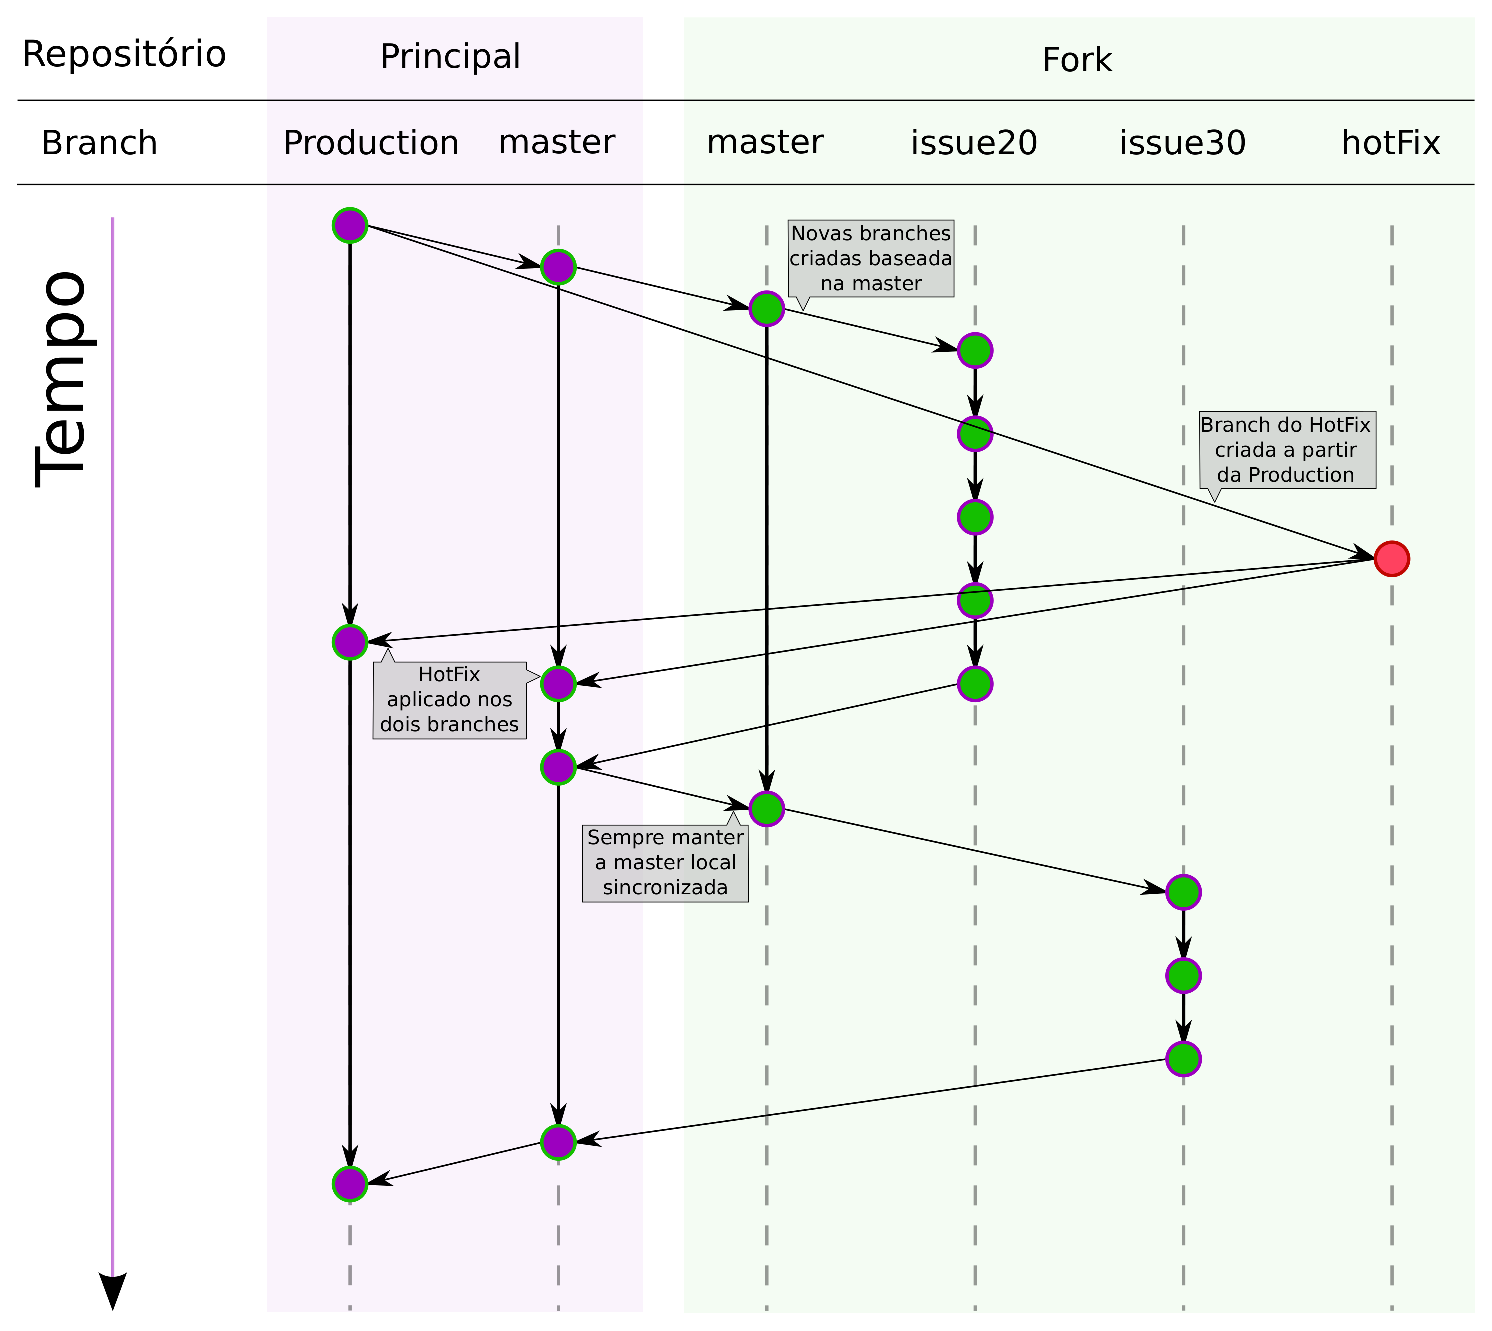
\includegraphics[scale=0.65]{./imagens/branchForkDiagram.eps}%
	\end{center}%
	\caption{10 maiores redes sociais em número de acessos no Brasil em novembro de 2104\label{fig:social-network-share-br}}%
	\fonte{Autoria Própria, baseado em \citeonline{serasa}}%
\end{figure}%

Na Figura \ref{fig:social-network-pensando} observamos as estatísticas de acesso, originados nas redes sociais, do projeto Pensando o Direito e das consultas públicas, com destaque especial para o Facebook com 90,91\% e para o Twitter com 7,1\%.
\begin{figure}[htb]%
	\begin{center}
		\begin{tikzpicture}
		  \begin{axis}[
		    xbar, xmin=0, xmax=105,
		    %grid=major,
		    width=12cm, height=12cm, enlarge y limits=0.1,
		    xlabel={\% de participação},
		    symbolic y coords={
			    {paper.li},
			    reddit,
			    Disqus,
			    {goo.gl},
			    Pocket,
			    LinkedIn,
			    Blogger,
			    Google+,
			    Twitter,
			    Facebook
		    },
		    ytick=data,
		    yticklabel style={/pgf/number format/fixed},
		    legend style={at={(0.12,-0.06)}, anchor=north,legend columns=-1},
		    nodes near coords, nodes near coords align={horizontal},
		    ]
		    %Pensando o Direito
		    \addplot
			[draw=black,pattern=horizontal lines dark blue]
		    coordinates {
			    (0.01,{paper.li})
			    (0.06,reddit)
			    (0.06,Disqus)
			    (0.13,{goo.gl})
			    (0.16,Pocket)
			    (0.18,LinkedIn)
			    (0.48,Blogger)
			    (0.9,Google+)
			    (7.10,Twitter)
			    (90.91,Facebook)
		    };
		  	\legend{Pensando}
		  \end{axis}
		\end{tikzpicture}
	\end{center}%
	\caption{10 redes sociais que mais direcionam acessos à plataforma Pensando O Direito\label{fig:social-network-pensando}}%
	\fonte{Autoria Própria baseado em estatísticas do Google Analytics}%
\end{figure}%

Na Figura \ref{fig:social-network-pensando-e-mercado} podemos observar a comparação entre as estatísticas de cotas do mercado brasileiro e as estatísticas do projeto Pensando o Direito. Como pode-se observar, o Facebook possui uma predominância muito maior no projeto Pensando O Direito (90,91\%) do que no mercado (64,82\%), assim como o Twitter (7,1\% no Pensando O Direito \textit{versus} 1,36\% no mercado).

Por outro lado, o Youtube sequer aparece nas estatísticas de origem de acesso do projeto Pensando O Direito, apesar de ser a segunda rede social mais acessada no Brasil com 26,04\% do mercado. Daqui percebe-se que um ponto importante a ser melhorado na comunicação do projeto Pensando O Direito seria trabalhar melhor a divulgação no YouTube. Para tanto, recomenda-se uma nova linha de ação na comunicação focada no Youtube, e que fossem produzidos vídeos de todos os projetos ligados ao Pensando O Direito concentrados numa única conta. Tambémé fundamental que na descrição de todos os vídeos existam links que remetam a páginas do projeto, ou de alguma consulta pública, ligadas ao vídeo.

Além de serem utilizados no próprio site do Pensando O Direito, estes vídeos também devem ser utilizados nas postagens e divulgações nas demais redes sociais, em especial no Facebook, sempre com links levando de volta ao site do Pensando O Direito.

\begin{figure}[htb]%
	\begin{center}
		\begin{tikzpicture}
		  \begin{axis}[
		    xbar, xmin=0, xmax=105,
		    %grid=major,
		    width=12cm, height=14cm, enlarge y limits=0.1,
		    xlabel={\% de participação},
		    symbolic y coords={LinkedIn,{Bate Papo UOL},Badoo,{Haboo Brasil},Instagram,Google+,Twitter,{Yahoo! Answers Brasil},Youtube,Facebook},
		    ytick=data,
		    legend style={at={(0.12,-0.05)}, anchor=north,legend columns=-1}, 
		    nodes near coords, nodes near coords align={horizontal},
		    ]
		    %Brasil
		    \addplot
			[draw=blue, pattern=horizontal lines light blue]
		    coordinates {
		    	(0.35,{Bate Papo UOL})
		    	(0.36,Badoo)
		    	(0.47,{Haboo Brasil})
		    	(0.54,Instagram)
		    	(0.70,Google+)
		    	(1.36,Twitter)
		    	(1.47,{Yahoo! Answers Brasil})
		    	(26.04,Youtube)
		    	(64.82,Facebook)
		    	(0.30,LinkedIn)
		    };
		    %Pensando o Direito
		    \addplot
			[draw=black,pattern=horizontal lines dark blue]
		    coordinates {
		    	(0,{Bate Papo UOL})
		    	(0,Badoo)
		    	(0,{Haboo Brasil})
		    	(0,Instagram)
		    	(0.90,Google+)
		    	(7.10,Twitter)
		    	(0,{Yahoo! Answers Brasil})
		    	(0,Youtube)
		    	(90.91,Facebook)
		    	(0.18,LinkedIn)
		    };
		  	\legend{Brasil, Pensando}
		  \end{axis}
		\end{tikzpicture}
	\end{center}%
	\caption{Comparação entre o percentual de acessos no Pensando O Direito e no Mercado\label{fig:social-network-pensando-e-mercado}}%
	\fonte{Autoria Própria baseado em estatísticas do Google Analytics e \citeonline{serasa}}%
\end{figure}%

\subsection{Comportamento dos usuários}
Para além da característica de número de acessos e suas origens, também é fundamental estudar outras características que podem ser obtidas das ferramentas de análises de visitantes, como o número de páginas por visita e o tempo médio de visita.

Na Figura \ref{fig:comportamento-redes-sociais} podemos observar que a duração média de uma sessão dos usuários advindos do Twitter (03m03s) é cerca de 78\% maior que a duração média de uma sessão dos usuários advindos do Facebook (01m43s). Além disso, podemos observar também que a quantidade de Páginas por Sessão dos usuários do Twitter (2,94) é 41\% maior que dos usuários vindos do Facebook (2,08).

\begin{figure}[htb]%
	\begin{center}
		\includegraphics[scale=0.55]{./imagens/comportamento-social.png}%
	\end{center}%
	\caption{Comportamento dos usuários do Pensando O Direito advindos das redes sociais\label{fig:comportamento-redes-sociais}}%
	\fonte{Google Analytics do site \url{http://participacao.mj.gov.br/}}%
\end{figure}%

Tomando por base as informações acima observadas, é razoável recomendar que haja um trabalho de divulgação mais focado e dedicado ao Twitter, sem prejuízo do trabalho realizado no Facebook. Como as ``linhas do tempo'' no Facebook não são completamente cronológicas e uma mesma postagem pode reaparecer na linha do tempo do usuário várias vezes ao dia, talvez uma única postagem diária seja suficiente para divulgação das iniciativas. Por outro lado, o Twitter possui uma linha do tempo completamente cronológica e, dessa forma, faz-se necessário um trabalho maior de postagens durante o dia \cite{killeen}, com mais de uma mensagem diária, para que se possa atingir um número maior de usuários. Outro característica distinta importante, é que o Twitter trabalha com mensagens mais curtas que o Facebook, então as postagens no Twitter poderiam ter uma característica mais focada numa pergunta direta com link levando à página aonde a pergunta deve ser respondida pelo usuário.

Existem ainda outros indicadores que poderiam ser avaliados na ferramenta de análise de visitantes, mas que não serão exploradas neste produto, como por exemplo os melhores horários para se postar em cada rede social, quais são os termos mais buscados que tem levado os usuários ao Pensando O Direito ou qual o Fluxo no site dos usuários advindos das redes sociais.

\subsection{Comentários advindos das redes sociais}
Uma tendência atual de integração de sites com as redes sociais é permitir que os usuários comentem nos conteúdos do site diretamente das redes sociais, sendo estes comentários apresentados no próprio site por meios das APIs das redes sociais.

A maior preocupação que se deve ter com esta abordagem é a falta de garantia de controle dos comentários em termos de armazenamento, para fins de registro histórico. Assumindo que este processo de consulta pública irá balizar decisões e ações governamentais, é fundamental garantir o registro das opiniões públicas que forem utilizadas.

Ademais, \citeonline{killeen} recomenda que sejam desenvolvidas cuidadosas políticas de privacidade, ``uso aceitável'' e de moderação para o website. \citeonline{brown} destaca ainda algumas características a serem avaliadas com relação às redes sociais utilizadas. Destas características, destacam-se:
\begin{inparaenum}[\itshape a\upshape)]
\item Segurança;
\item Questões legais relacionadas à mídia social, incluindo liberdade de expressão, liberdade de acesso à informação, divulgação pública, equidade de acesso, privacidade; e
\item regras de conduta permitidas da rede social.
\end{inparaenum}

\section{Redes Sociais Federadas Públicas}
Uma integração com redes sociais que poderia agregar muito ao caráter público e coletivo das plataformas é a integração com redes sociais federadas públicas já existentes, como o Participa.br. Essa integração poderia dar-se apenas em termos de login/cadastro dos usuários, compartilhando as bases de usuários das duas plataformas, favorecendo iniciativas de intercâmbio entre ambas plataformas.

Ainda assim, como o Participa.br utiliza tecnologias muito distintas do Pensando o Direito, Noofesro naquela e Wordpress nesta, uma integração mais completa, com comentários cruzados, é algo que demandaria um esforço que pode não compensar, mas a integração de login/usuários/cadastros já é mais simples, por meio de uma API, e poderia agregar muito a ambas plataformas.

\section{SEO}
Uma característica que precisa ser melhor trabalhada nas plataformas são os recursos de \gls{seo}. Algumas técnicas e características básicas de \gls{seo} foram aplicadas ao site atual, porém existem muitas outras que não o foram e que poderiam ajudar na divulgação do Pensando O Direito e seus projetos correlatos.

Neste ponto, recomenda-se buscar um especialista em técnicas avançadas de SEO, que não contemple apenas as ferramentas de busca tradicionais, mas também que conheça e possa recomendar técnicas que melhorem o desempenho das postagens nos perfis de redes sociais, como por exemplo a utilização de \textit{hashtags}.

\section{Podcast}
Outra opção que pode ajudar na disseminação das iniciativas da SAL/MJ e do Pensando O Direito seria a criação de um Podcast sobre as iniciativas e atividades, com uma página dedicada aos podcasts.

Estes podcasts poderiam tratar de pequenos pontos relativos às diversas temáticas tratadas pela SAL/MJ com uma divulgação periódica que ajude a ``fidelizar'' os usuários.
A duração e a periodicidade depender da capacidade de produção da equipe e isso deve ser levado em conta, mas recomenda-se uma periodicidade de uma semana. Sobre a duração existem diversos modelos, desde podcasts curtos, de 10 minutos, até podcasts mais longos, de 1 hora ou mais.

O objetivo desses podcasts seriam fazer uma pequena introdução sobre os diversos assuntos tratados na SAL, projetos de Lei acompanhados, ou mesmo pontos específicos de consultas públicas em andamento, no mesmo estilo das entrevistas realizadas durante a Consulta Pública do Marco Civil da Internet. A vantagem dos podcasts é que eles são mais leves e ``portáteis'', e os usuários podem simplesmente baixá-los e ouvi-los durante o dia, no trânsito, etc. Além de permitirem um debate um pouco mais aprofundado que os vídeos curtos já produzidos.

